\section{Perceptual Coding and MP3/AAC: Compression by Exploiting Human Hearing}

\subsection{Learning Objectives}

By the end of this lecture, you will be able to:
\begin{enumerate}[leftmargin=*, nosep]
    \item Explain why time-domain waveform coding is inefficient and why the frequency domain is the natural representation for perceptual audio coding.
    \item Describe the three pillars of the psychoacoustic model: the absolute threshold of hearing, simultaneous masking, and temporal masking.
    \item Define the Bark scale and critical bands, and explain their role in masking calculations.
    \item Explain the Modified Discrete Cosine Transform (MDCT) and why it is preferred over a plain DCT for audio signals.
    \item Trace the complete MP3 encoding pipeline: filterbank $\to$ MDCT $\to$ psychoacoustic model $\to$ bit allocation $\to$ quantisation $\to$ Huffman coding.
    \item Calculate the Signal-to-Mask Ratio (SMR) and determine which frequency bands can tolerate coarser quantisation.
    \item Identify and explain pre-echo, and describe how temporal masking and window switching mitigate it.
    \item Compare MP3 and AAC in terms of filterbank design, efficiency, and quality at low bit-rates.
    \item Connect the perceptual coding paradigm to the JPEG quality factor from the previous lecture.
\end{enumerate}

\subsection{Motivation: Why Is Audio Different from Images?}

\subsubsection{The Raw Cost of Digital Audio}

A single CD-quality audio signal requires:
\begin{itemize}[nosep]
    \item Sampling rate: 44,100 samples per second (slightly above the Nyquist requirement for the 20 Hz--20 kHz audible range)
    \item Bit depth: 16 bits per sample
    \item Channels: 2 (stereo)
\end{itemize}
The raw bit rate is calculated as:
\[
\text{Bit rate} = 44{,}100 \text{ samples/s} \times 16 \text{ bits/sample} \times 2 \text{ channels} = \mathbf{1{,}411{,}200 \text{ bits/s}} \approx 1.4\text{ Mbit/s}.
\]
One minute of CD-quality stereo audio occupies approximately 10 MB. Storing an album or streaming music over a dial-up modem would be completely impractical without compression.

\subsubsection{Why Not Just Use Lossless Compression?}

Lossless audio codecs (FLAC, Apple Lossless) achieve roughly 2:1 compression on typical music, reducing 1.4 Mbit/s to about 700 kbit/s. This is helpful but still far too large for real-time streaming over mobile networks or storing thousands of songs on portable devices. MP3 achieves 10:1 to 14:1 compression (128--320 kbit/s) \emph{while being perceptually transparent for many listeners under typical conditions}. The key question is: how?

\begin{importantbox}
\textbf{The Central Insight of Perceptual Coding:}
The human auditory system does not perceive all information in a sound signal equally. Large amounts of the signal can be discarded entirely without the listener being able to detect the loss. The goal of MP3 and AAC is not to minimise mathematical error (as in lossless coding) but to minimise \emph{perceptible} error. These are profoundly different objectives.
\end{importantbox}

\subsubsection{The Contrast with JPEG}

In the JPEG chapter we saw that the human visual system is less sensitive to high-frequency spatial detail. JPEG exploits this by quantising high-frequency DCT coefficients more coarsely. The psychoacoustic model in MP3 is the \emph{audio counterpart}: it determines, dynamically and per-frequency-band, how much quantisation noise the ear will tolerate at each instant in time. Both systems share the same three-stage skeleton:

\begin{center}
\begin{tikzpicture}[
    node distance=1.3cm,
    box/.style={draw, rounded corners=4pt, minimum width=2.8cm,
                minimum height=0.9cm, align=center, font=\small},
    lossless/.style={box, fill=blue!15, draw=blue!70!black},
    lossy/.style={box, fill=red!15, draw=red!70!black},
    arr/.style={-{Stealth[length=5pt]}, thick}
]
  \node[lossless] (T) {Transform\\(MDCT)};
  \node[lossy,  right=of T] (Q) {Perceptual\\Quantisation};
  \node[lossless,right=of Q] (E) {Huffman\\Coding};
  \draw[arr] (T)--(Q);
  \draw[arr] (Q)--(E);
  \node[below=0.2cm of T, font=\scriptsize\itshape, text=blue!70!black] {lossless};
  \node[below=0.2cm of Q, font=\scriptsize\bfseries,text=red!70!black]  {LOSSY};
  \node[below=0.2cm of E, font=\scriptsize\itshape, text=blue!70!black] {lossless};
  \node[above=0.6cm of Q, align=center, font=\scriptsize,
        text=red!60!black] {bit allocation driven by\\psychoacoustic model};
\end{tikzpicture}
\end{center}

The key difference from JPEG is the \textbf{psychoacoustic model}: an additional computational module that runs in parallel with the transform and dynamically tells the quantiser how many bits to assign to each frequency band.

\subsection{The Human Auditory System: Three Pillars of Perception}

\subsubsection{Pillar 1 — The Absolute Threshold of Hearing}

\begin{definitionbox}
\textbf{Absolute Threshold of Hearing (ATH):} The minimum sound pressure level (SPL) at each frequency that an average human can detect in a perfectly quiet environment. Any sound \emph{below} the ATH at a given frequency is completely inaudible and can be discarded at effectively zero perceptual cost.
\end{definitionbox}

The ATH is highly non-uniform across the audible spectrum. A useful approximation (Terhardt's formula) in dB SPL is:
\begin{equation}
T_{\text{ATH}}(f) = 3.64\left(\frac{f}{1000}\right)^{-0.8} - 6.5\,e^{-0.6(f/1000 - 3.3)^2} + 10^{-3}\!\left(\frac{f}{1000}\right)^4,
\label{eq:ath}
\end{equation}
where $f$ is in Hz and the result is in dB SPL.

\begin{figure}[H]
\centering
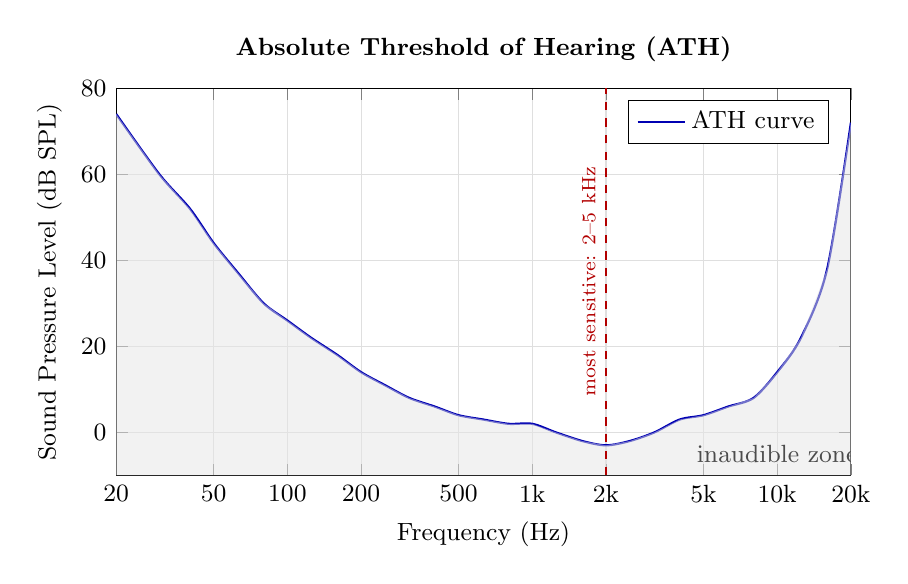
\begin{tikzpicture}
\begin{semilogxaxis}[
  width=0.9\textwidth, height=6.5cm,
  xlabel={Frequency (Hz)},
  ylabel={Sound Pressure Level (dB SPL)},
  xmin=20, xmax=20000,
  ymin=-10, ymax=80,
  grid=major, grid style={gray!25},
  xtick={20,50,100,200,500,1000,2000,5000,10000,20000},
  xticklabels={20,50,100,200,500,1k,2k,5k,10k,20k},
  label style={font=\small},
  tick label style={font=\small},
  title={Absolute Threshold of Hearing (ATH)},
  title style={font=\small\bfseries},
  legend pos=north east,
  legend style={font=\small},
  legend entries={ATH curve},
]
\addplot[blue!70!black, thick, smooth] coordinates {
  (20,74)  (30,60) (40,52) (50,44) (63,37) (80,30)
  (100,26) (125,22)(160,18)(200,14)(250,11)(315,8)
  (400,6)  (500,4) (630,3)(800,2)(1000,2)(1250,0)
  (1600,-2)(2000,-3)(2500,-2)(3150,0)(4000,3)(5000,4)
  (6300,6) (8000,8)(10000,14)(12500,22)(16000,38)(20000,72)
};
\addplot[fill=gray!20, draw=none, opacity=0.5] coordinates {
  (20,74)(30,60)(40,52)(50,44)(63,37)(80,30)
  (100,26)(125,22)(160,18)(200,14)(250,11)(315,8)
  (400,6)(500,4)(630,3)(800,2)(1000,2)(1250,0)
  (1600,-2)(2000,-3)(2500,-2)(3150,0)(4000,3)(5000,4)
  (6300,6)(8000,8)(10000,14)(12500,22)(16000,38)(20000,72)
  (20000,-10)(20,-10)
} -- cycle;
\draw[red!70!black, dashed, thick] (axis cs:2000,-10) -- (axis cs:2000,80);
\node[font=\scriptsize, text=red!70!black, rotate=90] at (axis cs:1700,35)
  {most sensitive: 2--5 kHz};
\node[font=\small, text=gray!60!black] at (axis cs:10000,-5)
  {inaudible zone};
\end{semilogxaxis}
\end{tikzpicture}
\caption{The Absolute Threshold of Hearing. The shaded region below the curve is completely inaudible. The ear is most sensitive around 3--4 kHz (where speech energy is concentrated) and rapidly loses sensitivity below 100 Hz and above 10 kHz. An MP3 encoder can assign \emph{effectively zero bits} to any frequency component whose level falls below this curve.}
\label{fig:ath}
\end{figure}

\begin{examplebox}
\textbf{Example 1: Using the ATH to discard frequency content for free.}

\medskip
Suppose a music signal has the following energy levels in three frequency bands:

\begin{center}
\begin{tabular}{lccc}
\toprule
Band & Frequency & Signal level (dB SPL) & ATH at that frequency \\
\midrule
A & 100 Hz  & 30 dB & 26 dB \\
B & 15 kHz  & 12 dB & 38 dB \\
C & 3 kHz   & 25 dB & $\approx 0$ dB \\
\bottomrule
\end{tabular}
\end{center}

\textbf{Step-by-step analysis, band by band:}

\textit{Band A (100 Hz, 30 dB):}
\begin{enumerate}[nosep]
    \item Compare signal to ATH: $30 \text{ dB} > 26 \text{ dB}$.
    \item The signal is 4 dB above the ATH, so it is audible.
    \item The encoder \emph{must} allocate bits here to represent it.
\end{enumerate}

\textit{Band B (15 kHz, 12 dB):}
\begin{enumerate}[nosep]
    \item Compare signal to ATH: $12 \text{ dB} < 38 \text{ dB}$.
    \item The signal is 26 dB \emph{below} the ATH.
    \item It is completely inaudible. The encoder allocates \textbf{effectively zero bits} to this band. (In practice, some minimal side information may still be transmitted, but no meaningful spectral energy is coded.) The listener cannot detect the omission.
\end{enumerate}

\textit{Band C (3 kHz, 25 dB):}
\begin{enumerate}[nosep]
    \item Compare signal to ATH: $25 \text{ dB} \gg 0 \text{ dB}$.
    \item It is clearly audible and well above the threshold.
    \item The encoder must allocate bits; moreover, errors here would be very perceptible, so quantisation must be fine.
\end{enumerate}

\textbf{Conclusion:} Without considering any masking at all, the ATH alone effectively eliminates Band B from the bit budget. In a typical music signal, the ATH makes a non-trivial fraction of the high-frequency content free to discard.
\end{examplebox}

\subsubsection{Pillar 2 — Simultaneous Masking (Frequency Masking)}

\begin{definitionbox}
\textbf{Simultaneous Masking:} When a loud \emph{masker} tone or narrow-band noise is present, it raises the hearing threshold in nearby frequency bands, making softer \emph{maskee} sounds inaudible even though they are above the ATH. Masking operates simultaneously in time (both sounds occur at the same moment) and spreads asymmetrically in frequency: a masker elevates the threshold more strongly \emph{above} its own frequency (upward spread) than below it.
\end{definitionbox}

\paragraph{Why does masking spread upward?}
The cochlea — the spiral, fluid-filled organ of the inner ear — separates sound by frequency along its length. A given frequency causes maximum vibration at a specific location (the \emph{basilar membrane travelling wave peak}). This vibration spreads more readily towards the high-frequency end because of the stiffness gradient of the basilar membrane. Hence a loud bass tone masks nearby mid-range tones more strongly than a high-pitched tone masks nearby bass tones.

\paragraph{Tonal vs. Noise Maskers}
It is important to distinguish between two types of maskers:
\begin{itemize}[nosep]
    \item \textbf{Tonal maskers:} Narrow spectral peaks (e.g., a pure tone or a single musical note). These produce strong, localised masking with a sharp spreading function.
    \item \textbf{Noise maskers:} Broad spectral humps (e.g., a drum hit, a cymbal crash, or background hiss). These produce weaker, broader masking because their energy is spread across many frequencies.
\end{itemize}
The MP3 psychoacoustic model classifies each spectral component as tonal or noise-like and applies different spreading functions accordingly.

\begin{figure}[H]
\centering
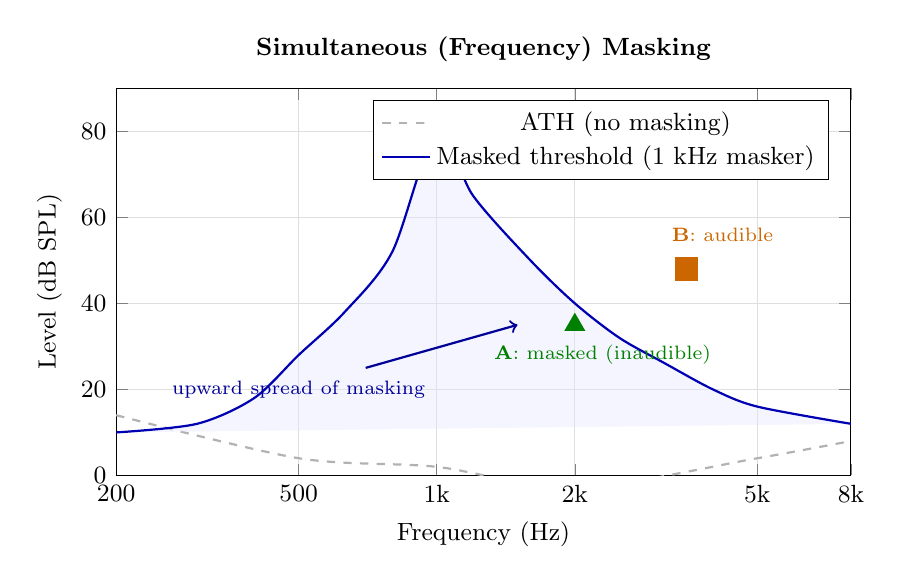
\begin{tikzpicture}
\begin{semilogxaxis}[
  width=0.9\textwidth, height=6.5cm,
  xlabel={Frequency (Hz)},
  ylabel={Level (dB SPL)},
  xmin=200, xmax=8000,
  ymin=0, ymax=90,
  grid=major, grid style={gray!25},
  xtick={200,500,1000,2000,5000,8000},
  xticklabels={200,500,1k,2k,5k,8k},
  label style={font=\small},
  tick label style={font=\small},
  title={Simultaneous (Frequency) Masking},
  title style={font=\small\bfseries},
  legend pos=north east,
  legend style={font=\small},
  legend entries={ATH (no masking), Masked threshold (1 kHz masker)},
]
\addplot[gray!60, thick, dashed, smooth] coordinates {
  (200,14)(500,4)(1000,2)(2000,-3)(5000,4)(8000,8)
};
\addplot[blue!70!black, thick, smooth, fill=blue!10, fill opacity=0.4] coordinates {
  (200,10)(300,12)(400,18)(500,28)(630,38)(800,52)
  (1000,80)
  (1200,65)(1600,50)(2000,40)(2500,32)(3150,26)
  (4000,20)(5000,16)(8000,12)
};
\addplot[red!80!black, mark=*, mark size=4pt, only marks] coordinates {(1000,80)};
\node[font=\small, text=red!80!black, right] at (axis cs:1050,80)
  {Masker: 1 kHz, 80 dB};
\addplot[green!50!black, mark=triangle*, mark size=4pt, only marks]
  coordinates {(2000,35)};
\node[font=\scriptsize, text=green!50!black, align=center] at (axis cs:2300,28)
  {\textbf{A}: masked (inaudible)};
\addplot[orange!80!black, mark=square*, mark size=4pt, only marks]
  coordinates {(3500,48)};
\node[font=\scriptsize, text=orange!80!black] at (axis cs:4200,56)
  {\textbf{B}: audible};
\node[font=\scriptsize, text=blue!60!black, align=center] at (axis cs:500,20)
  {upward spread of masking};
\draw[->, blue!60!black, thick] (axis cs:700,25) -- (axis cs:1500,35);
\end{semilogxaxis}
\end{tikzpicture}
\caption{Simultaneous (frequency) masking. A loud 1 kHz masker at 80 dB SPL raises the hearing threshold over a wide frequency range (blue curve). Maskee \textbf{A} at 2 kHz and 35 dB falls \emph{below} the masked threshold — it is completely inaudible despite being above the ATH. Maskee \textbf{B} at 3.5 kHz and 48 dB is above the masked threshold and therefore audible. Notice the asymmetry: masking spreads more strongly upward (to higher frequencies) than downward.}
\label{fig:simmasking}
\end{figure}

\begin{examplebox}
\textbf{Example 2: Computing the masking threshold and the SMR.}

\medskip
\noindent\textbf{Setup.} A 1 kHz pure tone masker has a level of 80 dB SPL. We want to know whether a 2 kHz tone at 35 dB SPL is audible.

\medskip
\noindent\textbf{Step 1 — Understand the spreading function concept.}
The ISO 11172-3 standard uses a detailed spreading model in Bark units (see Section~\ref{sec:bark}). In the vicinity of the masker, the masked threshold $T_m(f)$ is approximated by:
\[
T_m(f) \approx L_m - \Delta S(z_m, z),
\]
where $L_m = 80$ dB is the masker level, $z_m$ is the masker's Bark frequency, $z$ is the target Bark frequency, and $\Delta S$ is the attenuation of the spreading function (how much the masker's influence drops off as we move away in frequency).

\medskip
\noindent\textbf{Important note:} This is a simplified linear approximation for didactic purposes. Actual psychoacoustic models in MP3 and AAC use asymmetric, level-dependent spreading functions derived from extensive psychoacoustic experiments. The simplified version here captures the core idea without the complexity of the full ISO model.

\medskip
\noindent\textbf{Step 2 — Convert frequencies to Bark.}

We use the Bark conversion formula (Eq.~\eqref{eq:bark}) to get approximate values:
\[
z(1000\ \text{Hz}) \approx 8.5\ \text{Bark}, \qquad
z(2000\ \text{Hz}) \approx 13.0\ \text{Bark}.
\]
The distance in Bark units is $\Delta z = 13.0 - 8.5 = 4.5\ \text{Bark}$.

\medskip
\noindent\textbf{Step 3 — Apply the spreading function.}

For upward spread ($\Delta z > 0$), a standard didactic approximation is:
\[
\Delta S \approx (10 + 2.5\,\Delta z) \ \text{dB (for a tonal masker)}.
\]
Substituting the value:
\[
\Delta S = 10 + 2.5 \times 4.5 = 10 + 11.25 = 21.25\ \text{dB}.
\]
This means the masker's influence drops by 21.25 dB when we move from 1 kHz to 2 kHz.

\medskip
\noindent\textbf{Step 4 — Compute the masked threshold at 2 kHz.}
\[
T_m(2\ \text{kHz}) = L_m - \Delta S = 80 - 21.25 = 58.75\ \text{dB SPL}.
\]

\medskip
\noindent\textbf{Step 5 — Is the 2 kHz tone audible?}

The 2 kHz tone (the "maskee") has a level of 35 dB SPL. The masked threshold is 58.75 dB SPL. Since $35 < 58.75$, the tone is \textbf{completely masked} and inaudible. The encoder can allocate effectively zero bits to this frequency band without any perceptible degradation.

\medskip
\noindent\textbf{Step 6 — Compute the Signal-to-Mask Ratio (SMR).}

\begin{definitionbox}
\textbf{Signal-to-Mask Ratio (SMR):} The difference between the signal level and the masking threshold in a given frequency band:
\[
\mathrm{SMR}(f) = L_{\text{signal}}(f) - T_{\text{mask}}(f) \quad [\text{dB}].
\]
A negative SMR means the signal is masked (inaudible). A positive SMR means the signal is audible and the encoder must allocate bits to represent it, with more bits needed for a larger positive SMR.
\end{definitionbox}

Applying the definition:
\[
\mathrm{SMR}(2\ \text{kHz}) = L_{\text{signal}} - T_{\text{mask}} = 35 - 58.75 = -23.75\ \text{dB}.
\]

The negative value confirms the 2 kHz tone is masked. Conversely, if another band had $\mathrm{SMR}=+30\ \text{dB}$, it would be clearly audible and need fine quantisation (many bits).
\end{examplebox}

\subsubsection{The Bark Scale and Critical Bands}
\label{sec:bark}

The basilar membrane does not have uniform frequency resolution. Below about 500 Hz, frequency resolution is roughly constant in Hz (about 100 Hz wide per critical band). Above 500 Hz, resolution is roughly constant on a logarithmic scale, mirroring our perception of musical pitch. The \textbf{Bark scale} captures this non-linearity.

\begin{definitionbox}
\textbf{Critical Band:} The range of frequencies that activate the same region of the basilar membrane. Masking operates within and between critical bands. There are approximately 25 critical bands spanning the audible range 20 Hz--20 kHz.

\textbf{Bark Frequency:} A frequency scale calibrated to critical-band width. 1 Bark corresponds to approximately 1 critical-band width. A common conversion formula is:
\begin{equation}
z(f) = 13\arctan\!\left(0.00076\,f\right) + 3.5\arctan\!\left(\frac{f}{7500}\right)^2,
\label{eq:bark}
\end{equation}
where $f$ is in Hz and $z$ is in Bark. The function $\arctan$ returns a value in radians.
\end{definitionbox}

\begin{table}[H]
\centering
\caption{The 25 critical bands (Bark bands). Notice how the bandwidth in Hz grows with frequency while each band spans approximately 1 Bark. MP3 uses 32 subbands whose boundaries roughly align with these critical bands.}
\label{tab:bark}
\setlength{\tabcolsep}{8pt}
\begin{tabular}{cccc|cccc}
\toprule
Band & Lower (Hz) & Upper (Hz) & Width (Hz) &
Band & Lower (Hz) & Upper (Hz) & Width (Hz) \\
\midrule
1  &    20 &   100 &   80  & 14 & 2000 & 2320 &  320 \\
2  &   100 &   200 &  100  & 15 & 2320 & 2700 &  380 \\
3  &   200 &   300 &  100  & 16 & 2700 & 3150 &  450 \\
4  &   300 &   400 &  100  & 17 & 3150 & 3700 &  550 \\
5  &   400 &   510 &  110  & 18 & 3700 & 4400 &  700 \\
6  &   510 &   630 &  120  & 19 & 4400 & 5300 &  900 \\
7  &   630 &   770 &  140  & 20 & 5300 & 6400 & 1100 \\
8  &   770 &   920 &  150  & 21 & 6400 & 7700 & 1300 \\
9  &   920 &  1080 &  160  & 22 & 7700 & 9500 & 1800 \\
10 &  1080 &  1270 &  190  & 23 & 9500 &12000 & 2500 \\
11 &  1270 &  1480 &  210  & 24 &12000 &15500 & 3500 \\
12 &  1480 &  1720 &  240  & 25 &15500 &22050 & 6550 \\
13 &  1720 &  2000 &  280  &    &      &      &      \\
\bottomrule
\end{tabular}
\end{table}

\subsubsection{Pillar 3 — Temporal Masking}

\begin{definitionbox}
\textbf{Temporal Masking:} The masking effect extends \emph{in time} around a loud sound event, not just in frequency.
\begin{itemize}[nosep]
  \item \textbf{Post-masking (forward masking):} A loud sound continues to mask quieter sounds for up to 100--200 ms \emph{after} it ends. This occurs because the cochlea and auditory nerve need time to recover from the excitation.
  \item \textbf{Pre-masking (backward masking):} A loud sound masks quieter sounds up to 5--20 ms \emph{before} it begins. This seems paradoxical but arises because the brain integrates sound over a short time window (about 20-30 ms) before making a perceptual decision, effectively allowing a loud sound to "mask" sounds that occurred just before it.
\end{itemize}
\end{definitionbox}

\begin{figure}[H]
\centering
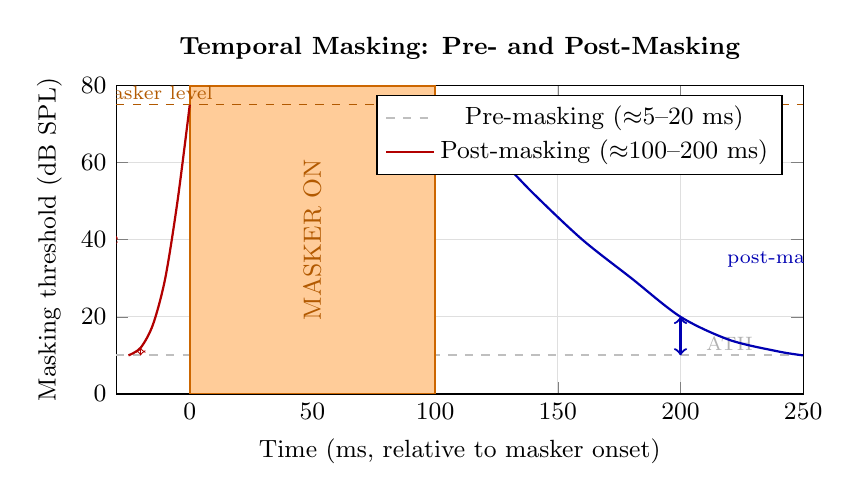
\begin{tikzpicture}
\begin{axis}[
  width=0.85\textwidth, height=5.5cm,
  xlabel={Time (ms, relative to masker onset)},
  ylabel={Masking threshold (dB SPL)},
  xmin=-30, xmax=250,
  ymin=0, ymax=80,
  grid=major, grid style={gray!25},
  label style={font=\small},
  tick label style={font=\small},
  title={Temporal Masking: Pre- and Post-Masking},
  title style={font=\small\bfseries},
  legend pos=north east,
  legend style={font=\small},
  legend entries={Pre-masking ($\approx$5--20 ms), Post-masking ($\approx$100--200 ms)},
]
\addplot[gray!50, dashed, thick] coordinates {(-30,10)(250,10)};
\node[font=\scriptsize, text=gray!60] at (axis cs:220,13) {ATH};
\fill[orange!40] (axis cs:0,0) rectangle (axis cs:100,80);
\draw[orange!80!black, thick] (axis cs:0,0) rectangle (axis cs:100,80);
\node[font=\small, text=orange!70!black, rotate=90] at (axis cs:50,40)
  {MASKER ON};
\addplot[red!70!black, thick, smooth] coordinates {
  (-25,10)(-20,12)(-15,18)(-10,30)(-5,50)(0,75)
};
\addplot[blue!70!black, thick, smooth] coordinates {
  (100,75)(120,65)(140,52)(160,40)(180,30)(200,20)(220,14)(240,11)(250,10)
};
\draw[orange!70!black, dashed] (axis cs:-30,75) -- (axis cs:250,75);
\node[font=\scriptsize, text=orange!70!black] at (axis cs:-15,78)
  {Masker level};
\draw[<->, red!70!black] (axis cs:-20,10) -- (axis cs:-20,12);
\node[font=\scriptsize, text=red!70!black, left, align=right] at (axis cs:-25,40)
  {pre-masking zone};
\draw[<->, blue!70!black, thick] (axis cs:200,10) -- (axis cs:200,20);
\node[font=\scriptsize, text=blue!70!black, right, align=left] at (axis cs:215,35)
  {post-masking zone};
\end{axis}
\end{tikzpicture}
\caption{Temporal masking. Before the masker starts (pre-masking), the threshold rises steeply over the last $\approx$20 ms. After the masker ends (post-masking), the threshold decays gradually over $\approx$200 ms. Any sound whose level falls below the temporal masking curve during these windows is inaudible. MP3's encoder uses this to allocate fewer bits to frames immediately following loud transients.}
\label{fig:temporal}
\end{figure}

\begin{importantbox}
\textbf{The Three Pillars Working Together:}
\begin{enumerate}[nosep]
  \item \textbf{ATH} sets a global noise floor below which everything is free.
  \item \textbf{Simultaneous masking} dynamically raises the threshold based on what loud signals are present right now, often by 20--60 dB.
  \item \textbf{Temporal masking} allows coarser coding in frames just before and after loud transients.
\end{enumerate}
Together these three effects mean that, for a typical music signal, the perceptual noise floor is often 40--60 dB higher than the ATH. The encoder can inject quantisation noise up to this raised floor without the listener detecting it. This is where the 10:1 compression ratio comes from.
\end{importantbox}

\subsection{The Modified Discrete Cosine Transform (MDCT)}

\subsubsection{Why Not the DCT?}

The plain DCT (as used in JPEG) computes 64 independent outputs from 64 independent inputs. If we apply this block by block to audio, adjacent blocks are processed independently. This creates the audio analogue of JPEG blocking artefacts: discontinuities at block boundaries that manifest as a ``flanging'' or ``warbling'' sound when converted back to the time domain.

A second problem is the trade-off between \textbf{frequency resolution} and \textbf{time resolution}. The psychoacoustic model needs to know the frequency content of the signal \emph{right now} (to compute accurate masking thresholds), but a longer block gives better frequency resolution at the cost of poorer temporal resolution. For stationary sounds (sustained notes), long blocks are ideal. For transients (drum hits, consonants in speech), short blocks are needed to track masking accurately and avoid pre-echo artefacts.

\subsubsection{The MDCT: Overlapping Blocks with Perfect Reconstruction}

\begin{definitionbox}
\textbf{Modified Discrete Cosine Transform (MDCT):} An overlapping transform where each block of $2N$ input samples produces $N$ output coefficients. Adjacent blocks overlap by 50\% (each sample appears in two consecutive transforms). Despite the overlap, the MDCT satisfies \textbf{perfect reconstruction}: the overlapping inverse MDCT (IMDCT) blocks, when added together using overlap-add, exactly recover the original signal (before quantisation).
\end{definitionbox}

\paragraph{MDCT formula.}
Given a windowed block of $2N$ samples $x(n)$, $n=0,\ldots,2N-1$:
\begin{equation}
X(k) = \sum_{n=0}^{2N-1} x(n)\,w(n)\, \cos\!\left(\frac{\pi}{N}\!\left(n+\frac{1}{2}+\frac{N}{2}\right) \left(k+\frac{1}{2}\right)\right), \quad k=0,\ldots,N-1,
\label{eq:mdct}
\end{equation}
where $w(n)$ is a carefully chosen analysis window (typically a sine window or Kaiser--Bessel derived window) that tapers to zero at the edges to ensure smooth overlap.

\paragraph{Key properties.}
\begin{enumerate}[nosep]
  \item \textbf{50\% overlap:} Each output frame of $N$ coefficients describes $2N$ input samples that overlap with the previous and next frames by $N$ samples.
  \item \textbf{Critical sampling:} Despite the overlap, the number of output coefficients ($N$) equals the number of \emph{new} input samples per frame ($N$), so no data expansion occurs.
  \item \textbf{TDAC property} (Time-Domain Aliasing Cancellation): The aliasing introduced by the overlap exactly cancels during the overlap-add reconstruction step, giving perfect reconstruction.
\end{enumerate}

\begin{figure}[H]
\centering
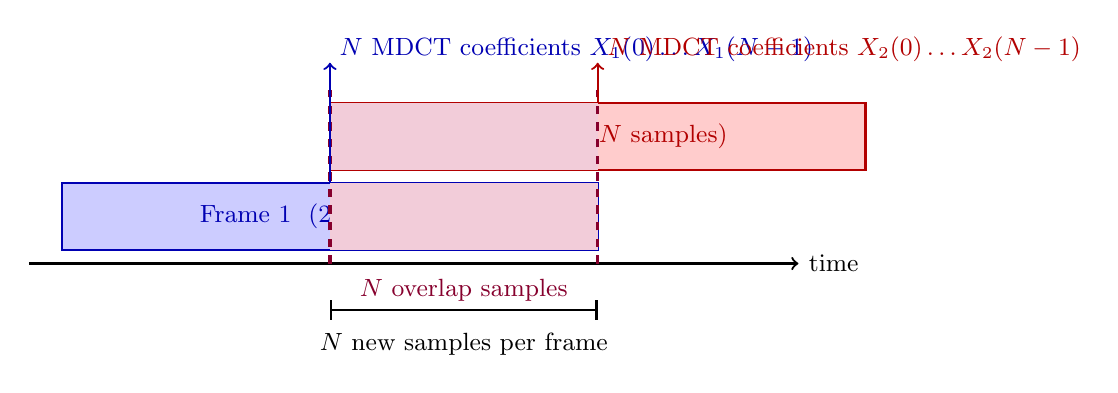
\begin{tikzpicture}[scale=0.85]
\draw[->, thick] (-0.5,0) -- (11,0) node[right, font=\small] {time};
\fill[blue!20] (0,0.2) rectangle (8,1.2);
\draw[blue!70!black, thick] (0,0.2) rectangle (8,1.2);
\node[font=\small, text=blue!70!black] at (4,0.7) {Frame 1 \ ($2N$ samples)};
\draw[blue!70!black, dashed, thick] (4,0) -- (4,0.2);
\fill[red!20] (4,1.4) rectangle (12,2.4);
\draw[red!70!black, thick] (4,1.4) rectangle (12,2.4);
\node[font=\small, text=red!70!black] at (8,1.9) {Frame 2 \ ($2N$ samples)};
\fill[purple!20] (4,0.2) rectangle (8,1.2);
\fill[purple!20] (4,1.4) rectangle (8,2.4);
\draw[purple!70!black, very thick, dashed] (4,0) -- (4,2.6);
\draw[purple!70!black, very thick, dashed] (8,0) -- (8,2.6);
\node[font=\small, text=purple!70!black] at (6,-0.4) {$N$ overlap samples};
\draw[->, thick, blue!70!black] (4,1.2) -- (4,3.0);
\node[font=\small, text=blue!70!black, right] at (4,3.2)
  {$N$ MDCT coefficients $X_1(0)\ldots X_1(N-1)$};
\draw[->, thick, red!70!black] (8,2.4) -- (8,3.0);
\node[font=\small, text=red!70!black, right] at (8,3.2)
  {$N$ MDCT coefficients $X_2(0)\ldots X_2(N-1)$};
\draw[|-|, thick] (4,-0.7) -- (8,-0.7);
\node[font=\small, below] at (6,-0.9) {$N$ new samples per frame};
\end{tikzpicture}
\caption{MDCT overlapping frames. Each frame of $2N$ input samples produces $N$ MDCT coefficients (critical sampling). Adjacent frames overlap by $N$ samples (50\%). Despite the overlap, the inverse MDCT with overlap-add perfectly reconstructs the original signal (before quantisation). This greatly reduces the blocking artefacts that would occur with non-overlapping blocks.}
\label{fig:mdct_overlap}
\end{figure}

\subsubsection{Window Switching: Handling Transients}

For stationary signals (sustained notes), MP3 uses \textbf{long blocks} ($N=576$ frequency lines from $2\times576=1152$ input samples), giving fine frequency resolution (suitable for accurate masking calculation).

When a sharp transient is detected (e.g., a drum hit), the encoder switches to \textbf{short blocks} ($N=192$ frequency lines from $2\times192=384$ input samples), giving finer time resolution. This is critical to avoid \textbf{pre-echo}.

\begin{warningbox}
\textbf{Pre-Echo: The Most Audible MP3 Artefact at Low Bit-Rates.}

Consider encoding a sudden drum hit using a long block of 1152 samples ($\approx 26$ ms at 44.1 kHz). The psychoacoustic model calculates masking thresholds for the \emph{entire block}, which is dominated by the loud portion after the transient. It therefore permits a high noise floor throughout the block.

However, quantisation noise is spread across the entire block after the inverse transform (the noise is uniform in the transform domain but becomes distributed in time after the IMDCT and overlap-add). The 26 ms of \emph{silence before} the drum hit (which had no masking) now contains audible noise — you hear a faint ``pre-echo'' of the drumstick before the drum has even been struck.

\textbf{Solution:} Switch to short blocks when a transient is detected. Each short block spans only $\approx 8.7$ ms, so quantisation noise cannot spread more than 8.7 ms before the transient. Post-masking from the loud transient then hides any noise in the preceding short block.
\end{warningbox}

\subsection{The Complete MP3 Encoding Pipeline}

\begin{figure}[H]
\centering
\begin{tikzpicture}[
    node distance=0.4cm and 0.5cm,
    block/.style={draw, rounded corners=4pt, minimum width=2.0cm,
                  minimum height=0.8cm, align=center, font=\scriptsize},
    input/.style={block, fill=gray!15,    draw=gray!60},
    filt/.style= {block, fill=blue!15,   draw=blue!70!black},
    mdct/.style= {block, fill=blue!20,   draw=blue!70!black},
    psych/.style={block, fill=orange!20, draw=orange!70!black},
    quant/.style={block, fill=red!15,    draw=red!70!black},
    ent/.style=  {block, fill=green!15,  draw=green!50!black},
    arr/.style={-{Stealth[length=4pt]}, thick}
]
  \node[input]  (pcm)   {PCM\\Input};
  \node[filt,   right=of pcm]  (pqmf) {Polyphase\\Filterbank};
  \node[mdct,   right=of pqmf] (mdct) {MDCT\\(long/short)};
  \node[quant,  right=of mdct] (qnt)  {Quantise\\+ Scale};
  \node[ent,    right=of qnt]  (huf)  {Huffman\\Coding};
  \node[input,  right=of huf]  (bs)   {Bitstream\\Output};
  \node[psych, below=1.2cm of pqmf] (fft)  {FFT\\Analysis};
  \node[psych, right=of fft]        (psy)  {Psychoacoustic\\Model};
  \node[psych, right=of psy]        (ba)   {Bit\\Allocation};
  \foreach \a/\b in {pcm/pqmf, pqmf/mdct, mdct/qnt, qnt/huf, huf/bs}
    \draw[arr] (\a)--(\b);
  \draw[arr] (pcm.south) |- (fft.west);
  \draw[arr] (fft)--(psy);
  \draw[arr] (psy)--(ba);
  \draw[arr] (ba.north) -- (qnt.south);
  \node[above=0.5cm of pqmf, font=\scriptsize\itshape, text=blue!70!black]
    {32 subbands};
  \node[above=0.5cm of mdct, font=\scriptsize\itshape, text=blue!70!black]
    {576 freq.\ lines};
  \node[above=0.5cm of qnt, font=\scriptsize\bfseries, text=red!70!black]
    {LOSSY};
  \node[below=0.3cm of psy, font=\scriptsize, text=orange!70!black]
    {masking thresholds};
  \node[below=0.3cm of ba, font=\scriptsize, text=orange!70!black]
    {bits per band};
\end{tikzpicture}
\caption{Complete MP3 encoding pipeline. The top path is the main audio processing chain. The bottom path is the psychoacoustic model, which runs in parallel (using an FFT for high-resolution spectral analysis) and feeds the bit allocation module. Only the quantisation stage is irreversible.}
\label{fig:mp3pipeline}
\end{figure}

\subsubsection{Stage 1 — Polyphase Quadrature Mirror Filterbank (PQMF)}

The MP3 encoder first divides the audio into 32 equal-width subbands using a \textbf{polyphase quadrature mirror filterbank}. Nominally, each subband spans $22{,}050/32 \approx 689$ Hz (for a 44.1 kHz signal), but with significant overlap due to non-ideal filter responses (real-world filters have finite roll-off, so energy leaks between adjacent bands).

Each subband produces 18 samples per frame for each of 32 subbands, giving $32\times18=576$ values per frame. These 576 values are then transformed by the MDCT.

\begin{importantbox}
\textbf{Why two stages (filterbank then MDCT)?}
This hybrid structure (called the \emph{hybrid filterbank}) is an MP3-specific design choice. The 32-band PQMF was inherited from the earlier MPEG-1 Layer I and II standards (which did not use MDCT). Adding the MDCT on top of each subband effectively gives $32\times18=576$ frequency lines, which is sufficient frequency resolution for an accurate psychoacoustic model. AAC replaces this two-stage hybrid with a single MDCT, which is architecturally cleaner and avoids the aliasing artefacts of the PQMF.
\end{importantbox}

\subsubsection{Stage 2 — Psychoacoustic Analysis (in Parallel)}

While the filterbank and MDCT process the main audio path, a separate \textbf{1024-point FFT} analyses the same PCM samples to produce a high-resolution power spectrum. This is used because the FFT provides finer frequency resolution than the MDCT alone.

From the FFT spectrum, the psychoacoustic model:
\begin{enumerate}[nosep]
  \item Identifies tonal maskers (narrow spectral peaks) and noise maskers (broad spectral humps).
  \item Computes the spreading function for each masker across all Bark bands.
  \item Sums all masking contributions to obtain a total masking threshold $T(f)$ for each frequency band.
  \item Combines $T(f)$ with the ATH (taking the higher of the two).
  \item Computes the SMR for each subband.
\end{enumerate}

\subsubsection{Stage 3 — Bit Allocation}

The bit allocator uses the SMR values to decide how many bits to assign to each subband. The guiding principle is:

\begin{definitionbox}
\textbf{Noise Shaping Objective:} Allocate bits such that the quantisation noise in each band is just below the masking threshold — no more, no less. Allocating more bits than needed wastes the bit budget; allocating fewer makes the noise audible.

The psychoacoustic model effectively defines a distortion measure: distortion is perceptually acceptable as long as the quantisation noise remains below the masking threshold.
\end{definitionbox}

MP3 uses an iterative \textbf{analysis-by-synthesis} bit allocation loop (the ``outer iteration''):
\begin{enumerate}[nosep]
  \item Start with effectively zero bits in all bands.
  \item Quantise all MDCT coefficients at the current quantisation levels.
  \item Check: does any band have audible quantisation noise (noise above masking threshold)?
  \item If yes, increase bits for the worst offending band and go to step 2.
  \item Repeat until all bands have noise below threshold, or the bit budget (target bit-rate) is exhausted.
\end{enumerate}

Additionally, MP3 employs a \textbf{bit reservoir} mechanism: it can borrow bits from neighbouring frames (when they are easy to code) to allocate more bits to complex segments, and return the borrowed bits later. This improves quality during transient-heavy passages.

\begin{examplebox}
\textbf{Example 3: Bit allocation across five frequency bands.}

\medskip
\noindent Suppose the psychoacoustic model has computed the following for five subbands of a music frame. The masking threshold is given in dB relative to the maximum signal level.

\begin{center}
\setlength{\tabcolsep}{7pt}
\begin{tabular}{lcccccc}
\toprule
Band & Frequency & Signal & Masking  & SMR     & Required  & Bits \\
     & (Hz)      & (dB)   & thr. (dB)& (dB)    & SNR (dB)  & needed \\
\midrule
1 & 0--700    & 70 & 55 & $+15$ & 15 & $\lceil 15/6 \rceil = 3$ \\
2 & 700--1400 & 80 & 30 & $+50$ & 50 & $\lceil 50/6 \rceil = 9$ \\
3 & 1400--2100& 60 & 65 & $-5$  & 0  & 0 (masked!) \\
4 & 2100--2800& 45 & 10 & $+35$ & 35 & $\lceil 35/6 \rceil = 6$ \\
5 & 2800--3500& 20 & 38 & $-18$ & 0  & 0 (below ATH!) \\
\bottomrule
\end{tabular}
\end{center}

\textbf{Step-by-step reasoning:}

\medskip
\noindent\textit{Band 1 (0--700 Hz):}
The signal is 15 dB above the masking threshold. Each bit of quantisation provides approximately 6 dB of signal-to-noise ratio (SNR) (the 6 dB/bit rule, see Section 3.6). We need enough bits to make the quantisation noise quieter than the masking threshold. We approximate the required SNR as being equal to the SMR for the purpose of bit allocation intuition. We need at least $15/6 = 2.5$ bits, so we allocate 3 bits.

\medskip
\noindent\textit{Band 2 (700--1400 Hz):}
The signal is 50 dB above the masking threshold. This is a loud, clearly audible band — perhaps the main melody. We need $50/6 \approx 8.3$ bits, so we allocate 9 bits. This band gets the most bits because it has the highest SMR.

\medskip
\noindent\textit{Band 3 (1400--2100 Hz):}
The signal is 5 dB \emph{below} the masking threshold (SMR $= -5$ dB). Even without any coding, the signal here is already inaudible because it is being masked by the loud Band 2 signal. \textbf{Effectively zero bits allocated.}

\medskip
\noindent\textit{Band 4 (2100--2800 Hz):}
The signal is 35 dB above the threshold. We need $35/6 \approx 5.8$ bits, so we allocate 6 bits.

\medskip
\noindent\textit{Band 5 (2800--3500 Hz):}
The signal level (20 dB) is below the ATH (38 dB at this frequency). It is completely inaudible even without masking. \textbf{Effectively zero bits allocated.}

\medskip
\noindent\textbf{Total bits used:} $3+9+0+6+0=18$ bits for this frame across these five bands. Without the psychoacoustic model, a naive coder might allocate roughly 9--10 bits to each band to ensure high fidelity, totalling $5\times10=50$ bits. The model achieves a $50/18\approx2.8\times$ additional reduction on top of whatever the MDCT already provides.
\end{examplebox}

\subsubsection{Stage 4 — Quantisation and Huffman Coding}

The MDCT coefficients are quantised using a non-uniform scalar quantiser. Unlike JPEG (which uses different step sizes per coefficient), MP3 applies a global \emph{scalefactor} to each subband before uniform quantisation:

\begin{equation}
\hat{X}(k) = \operatorname{nint}\!\left( \frac{|X(k)|^{3/4}}{\text{quantstep}} \right) \times \operatorname{sgn}(X(k)),
\label{eq:mp3quant}
\end{equation}

where $\operatorname{nint}$ denotes rounding to the nearest integer. This nonlinearity (the $3/4$ power law) approximates perceptual loudness scaling (the ear's sensitivity follows a power law, roughly $x^{0.6}$ to $x^{0.8}$). Using $|X(k)|^{3/4}$ makes the quantiser step size grow nonlinearly with coefficient amplitude, matching the ear's reduced sensitivity to quantisation error in loud sounds. This improves coding efficiency compared to a uniform quantiser.

The quantised values are then Huffman coded using one of 32 predefined Huffman tables (selected based on the statistics of the quantised values in each region of the spectrum). Big values (high-amplitude coefficients) use different tables from small values, and coefficients that are zero are run-length encoded — directly analogous to JPEG's End-of-Block (EOB) mechanism.

\subsection{Pre-Echo and Window Switching: A Detailed Example}

\begin{examplebox}
\textbf{Example 4: Pre-Echo — Why Transients Demand Special Treatment.}

\medskip
\noindent\textbf{Scenario.} A drum hit occurs at sample 800 within a 1152-sample long block (at 44.1 kHz, 1152 samples $\approx 26$ ms). Samples 0--799 are near-silence; samples 800--1151 contain the percussive attack.

\medskip
\noindent\textbf{Step 1 — Masking calculation with a long block.}

The psychoacoustic model analyses the entire 1152-sample block. The FFT is dominated by the loud transient in samples 800--1151. The model computes a high masking threshold of, say, 55 dB across most frequency bands, reflecting the loudness of the drum.

\medskip
\noindent\textbf{Step 2 — Bit allocation with a long block.}

The bit allocator sees high masking thresholds and allocates relatively few bits to the low-frequency bands (the drum masks them). This is correct for samples 800--1151, where the drum is loud.

\medskip
\noindent\textbf{Step 3 — Quantisation with a long block.}

With few bits allocated, quantisation is coarse — say, a step size of 32. The quantisation error is uniform in the MDCT coefficient domain, but after the inverse MDCT and overlap-add, it becomes distributed across the entire time-domain block. This means samples 0--799 (the silence before the drum) will contain quantisation noise.

We can estimate the quantisation noise power. For a uniform quantiser with step size $\Delta$, the noise power is $\sigma_q^2 = \Delta^2 / 12$. With $\Delta = 32$, the noise power is $\sigma_q^2 \approx 32^2/12 \approx 85.3$. This corresponds to a noise level of $10\log_{10}(85.3)\approx 19.3$ dB relative to a unit-amplitude signal.

\medskip
\noindent\textbf{Step 4 — The problem.}

In samples 0--799 (the silence), the signal level is near zero — say, $-50$ dB relative to full scale. The masking threshold in this region should be close to the ATH, around $0$--$10$ dB SPL. But our quantisation noise is at $\approx19$ dB SPL.

\[
\text{Noise level } (19\ \text{dB}) \gg \text{Masking threshold }(10\ \text{dB})
\]

The noise in the silence before the drum is \textbf{clearly audible}. This is the pre-echo artefact: you hear a ghost of the drum before the drum strikes.

\medskip
\noindent\textbf{Step 5 — Solution: switch to short blocks.}

The transient detector flags the onset of the drum hit. The encoder switches to 3 short blocks, each spanning $384$ samples ($\approx 8.7$ ms). The blocks cover the original long block's duration:

\begin{center}
\begin{tabular}{lcc}
\toprule
Short block & Samples & Content \\
\midrule
Block A & 0--383   & silence \\
Block B & 384--767 & silence + onset \\
Block C & 768--1151& full attack \\
\bottomrule
\end{tabular}
\end{center}

Each short block is quantised independently.
- For Block A (silence), the masking threshold is low, so the bit allocator assigns many bits to keep noise below the ATH.
- For Block C (loud attack), the masking threshold is high and the signal is loud — the allocator can be generous with noise and still keep it inaudible.
- Block B contains the transition. Post-masking from the loud Block C will hide any noise introduced in Block B.

Quantisation noise is now confined to 8.7 ms windows. The pre-echo is eliminated because the noise cannot spread far into the silence.

\medskip
\noindent\textbf{Trade-off.} Short blocks give poorer frequency resolution (fewer MDCT lines per block), reducing the precision of the psychoacoustic model. Window switching therefore uses short blocks only when a transient is detected, returning to long blocks for sustained sounds.
\end{examplebox}

\subsection{AAC: The Successor to MP3}

\subsubsection{Architectural Improvements}

Advanced Audio Coding (AAC, ISO/IEC 14496-3) was standardised in 1997 as the direct successor to MP3. It achieves better quality at the same bit-rate (or equivalent quality at a lower bit-rate) through several key changes:

\begin{table}[H]
\centering
\caption{MP3 vs.\ AAC: architectural comparison.}
\label{tab:mp3vsaac}
\setlength{\tabcolsep}{5pt}
\begin{tabular}{lll}
\toprule
\textbf{Feature} & \textbf{MP3 (MPEG-1 Layer III)} & \textbf{AAC (MPEG-4 Part 3)} \\
\midrule
Filterbank & Hybrid: 32-band PQMF + MDCT & Pure MDCT only \\
MDCT size (long) & 576 lines & 1024 or 2048 lines (depending on profile) \\
MDCT size (short) & 192 lines & 128 or 256 lines \\
Channels & Up to 2 (stereo) & Up to 48 \\
Huffman tables & 32 fixed tables & Adaptive tables (can be changed per frame) \\
Joint stereo & Simple M/S stereo & M/S + intensity stereo (replaces high-freq S with scaled M) \\
Temporal noise shaping & No & Yes (TNS) \\
Perceptual noise substitution & No & Yes (PNS) \\
Max bit-rate & 320 kbit/s & 576 kbit/s per channel (in Main profile) \\
Typical transparent quality & 192--256 kbit/s & 128--160 kbit/s \\
\bottomrule
\end{tabular}
\end{table}

\subsubsection{The Pure MDCT Filterbank}

AAC's most important improvement is replacing MP3's hybrid filterbank with a single MDCT operating directly on the PCM samples. This gives:

\begin{enumerate}[nosep]
  \item \textbf{1024 frequency lines} (vs.\ MP3's 576), giving $1024/576\approx1.8\times$ better frequency resolution for the psychoacoustic model.
  \item No aliasing cancellation errors from the PQMF stage, leading to a cleaner signal.
  \item Cleaner implementation and faster encoding.
\end{enumerate}

\subsubsection{Temporal Noise Shaping (TNS)}

TNS is an AAC-specific tool that addresses a fundamental limitation: the psychoacoustic model works in the frequency domain but quantisation noise is spread across the time-domain block after the inverse transform.

\begin{definitionbox}
\textbf{Temporal Noise Shaping (TNS):} Applies a prediction filter to the MDCT coefficients \emph{in the frequency domain}, which has the effect of shaping the quantisation noise \emph{in the time domain}. By applying a filter that concentrates energy in the frequency domain, TNS causes the noise to be concentrated at the portion of the time-domain block where the signal is loudest — where masking is strongest. This directly attacks the pre-echo problem without requiring window switching.
\end{definitionbox}

\subsubsection{Joint Stereo Coding}

For stereo signals, both MP3 and AAC exploit correlations between the left and right channels. Instead of coding L and R independently, they code:
\[
M = \frac{L+R}{2} \quad \text{(mid/sum channel)}, \qquad
S = \frac{L-R}{2} \quad \text{(side/difference channel)}.
\]
For a typical music signal, most energy is in $M$ (both channels play similar content). The $S$ channel (the difference) often has very little energy and can be quantised coarsely or omitted at low bit-rates. This \textbf{M/S stereo} scheme typically saves 10--25\% of the bit budget compared to independent L/R coding.

\begin{examplebox}
\textbf{Example 5: Mid/Side Stereo Coding.}

\medskip
A 1 kHz sine wave is recorded in stereo. Left and right channels:
\[
L(t) = 0.8\sin(2\pi\cdot1000t), \qquad
R(t) = 0.7\sin(2\pi\cdot1000t).
\]

\noindent\textbf{Step 1 — Compute M and S.}
\[
M(t) = \frac{L+R}{2} = \frac{0.8+0.7}{2}\sin(2\pi\cdot1000t) = 0.75\sin(2\pi\cdot1000t),
\]
\[
S(t) = \frac{L-R}{2} = \frac{0.8-0.7}{2}\sin(2\pi\cdot1000t) = 0.05\sin(2\pi\cdot1000t).
\]

\noindent\textbf{Step 2 — Compare energy.}
For a sine wave, the power is proportional to the square of the amplitude. We can compare the energies:
\[
E_M \propto 0.75^2 = 0.5625, \qquad E_S \propto 0.05^2 = 0.0025.
\]
Thus, $E_M / E_S = 0.5625 / 0.0025 = 225$, i.e., the mid channel has \textbf{225 times more energy} than the side channel.

\noindent\textbf{Step 3 — Bit allocation.}

Suppose the total bit budget for this frequency band is 10 bits. With independent L/R coding, we might allocate 5 bits to L and 5 bits to R. With M/S stereo, we allocate bits based on energy and perceptual importance:
\begin{itemize}[nosep]
  \item 8 bits to $M$ (high energy, perceptually important)
  \item 2 bits to $S$ (low energy; even coarse quantisation is barely audible)
\end{itemize}

The $M$ channel is reconstructed with high fidelity. The $S$ channel has coarser quantisation, but since $E_S$ is tiny, the resulting error in L and R is very small:
\[
L = M + S,\ \ \ R = M - S.
\]
Any quantisation error in $M$ ($\Delta M$) and $S$ ($\Delta S$) affects the reconstructed channels as:
\[
\Delta L = \Delta M + \Delta S, \qquad \Delta R = \Delta M - \Delta S.
\]
If $\Delta S$ is small (due to coarse quantisation but a small signal), both $\Delta L$ and $\Delta R$ are dominated by the high-quality $\Delta M$ term.

\noindent\textbf{Conclusion:} M/S stereo gives better overall quality than independent L/R coding when the two channels are strongly correlated, which is the typical case for popular music.
\end{examplebox}

\subsection{The 6 dB/Bit Rule and Rate--Distortion in Audio}

\subsubsection{Quantisation Noise and Bit Depth}

For a uniform quantiser with step size $\Delta$, the quantisation noise power is:
\begin{equation}
\sigma_q^2 = \frac{\Delta^2}{12}.
\end{equation}

If we use $b$ bits to represent a coefficient with peak amplitude $A$, then $\Delta = 2A/2^b$. Assuming the signal power $\sigma_{\text{signal}}^2$ is proportional to $A^2$, the Signal-to-Quantisation-Noise Ratio (SNR) is:
\begin{equation}
\mathrm{SNR} = \frac{\sigma_{\text{signal}}^2}{\sigma_q^2} \approx \frac{A^2}{(2A/2^b)^2/12} = \frac{3}{2} \cdot 2^{2b}.
\end{equation}
In decibels, this is:
\begin{equation}
\mathrm{SNR_{dB}} = 10 \log_{10}\left(\frac{3}{2}\right) + 10 \log_{10}(2^{2b}) \approx 1.76 + 6.02b \ \text{[dB]}.
\label{eq:snrbit}
\end{equation}
This is the famous \textbf{6 dB per bit rule}: each additional bit of quantisation improves SNR by approximately 6 dB.

\begin{examplebox}
\textbf{Example 6: The 6 dB/bit rule in practice.}

\medskip
A subband has an SMR of 42 dB. How many bits are needed?

\medskip
\noindent\textbf{Step 1.} We need the SNR of our quantisation to be at least 42 dB to keep the quantisation noise power below the masking threshold power.

\medskip
\noindent\textbf{Step 2.} Using Eq.~\eqref{eq:snrbit}, we ignore the constant 1.76 dB as a safety margin, giving the simplified formula $\mathrm{SNR_{dB}} \approx 6b$:
\[
b \ge \frac{42}{6} = 7 \ \text{bits}.
\]
A more precise calculation using $6.02b$ would give $b \ge 42/6.02 \approx 6.98$, so $b = 7$ bits is still sufficient.

\medskip
\noindent\textbf{Step 3.} Verify: $7 \times 6.02 = 42.14$ dB $\ge 42$ dB. \checkmark

\medskip
If instead SMR $=12$ dB: $b = \lceil12/6\rceil = 2$ bits only. At 16 bits per sample (CD quality), we allocate only 2 bits in this band instead of 16 — an 8:1 reduction in this band alone.

\medskip
\noindent\textbf{The whole game in one sentence:} MP3 looks at what the ear can hear in each frequency band at each moment, and allocates just enough bits to keep noise below that threshold — not one bit more.
\end{examplebox}

\subsection{Worked End-to-End Example: One MP3 Frame}

\begin{examplebox}
\textbf{Example 7: Tracing one MP3 frame from PCM to bitstream.}

\medskip
\noindent We trace a single granule (half a frame) of MP3 encoding for a simple two-tone signal. The signal contains a 1 kHz tone at 80 dB SPL and a 2 kHz tone at 30 dB SPL, sampled at 44.1 kHz, stereo (but we analyse only the left channel for brevity).

\medskip
\noindent\textbf{Stage 1 — Polyphase filterbank.}

The 1152-sample PCM block is fed into the 32-band PQMF. After the filterbank:
\begin{itemize}[nosep]
  \item Subband 1 (0--689 Hz): contains mainly the 1 kHz tone. \textit{Energy: high.}
  \item Subband 2 (689--1378 Hz): also contains 1 kHz tone (note: the PQMF has finite roll-off so energy leaks between adjacent bands). \textit{Energy: medium.}
  \item Subband 3 (1378--2067 Hz): contains the 2 kHz tone. \textit{Energy: low.}
  \item Subbands 4--32: no signal. \textit{Energy: negligible.}
\end{itemize}

\medskip
\noindent\textbf{Stage 2 — MDCT.}

Each subband's 18 samples undergo an 18-point MDCT, producing 18 MDCT coefficients per subband. For subbands 1 and 2, the MDCT coefficients at the tone frequency have large values; all other coefficients are near zero (good energy compaction). For subbands 4--32, all 18 coefficients are near zero.

Total non-negligible MDCT coefficients: $\approx 6$ (2 subbands $\times$ 3 significant lines each), out of $32\times18=576$ total.

\medskip
\noindent\textbf{Stage 3 — Psychoacoustic model.}

The FFT analysis of the same PCM block reveals two peaks:
\begin{center}
\begin{tabular}{cccc}
\toprule
Peak & Frequency & Level & Type \\
\midrule
A & 1 kHz & 80 dB & tonal masker \\
B & 2 kHz & 30 dB & tonal maskee \\
\bottomrule
\end{tabular}
\end{center}

Masking calculation (using the method of Example 2):
\begin{itemize}[nosep]
  \item Distance in Bark: $z(2\ \text{kHz}) - z(1\ \text{kHz}) \approx 13.0 - 8.5 = 4.5$ Bark.
  \item Upward spread attenuation: $\Delta S = 10 + 2.5\times4.5 = 21.25$ dB.
  \item Masked threshold at 2 kHz: $80 - 21.25 = 58.75$ dB SPL.
  \item Signal at 2 kHz: 30 dB SPL.
  \item SMR at 2 kHz: $30 - 58.75 = -28.75$ dB.
\end{itemize}
The 2 kHz tone is masked.

\medskip
\noindent\textbf{Stage 4 — Bit allocation.}

\begin{center}
\setlength{\tabcolsep}{6pt}
\begin{tabular}{lcccc}
\toprule
Region & Signal & Masking thr. & SMR & Bits allocated \\
\midrule
1 kHz (subbands 1--2) & 80 dB & 10 dB (ATH) & $+70$ dB & $\lceil70/6\rceil=12$ \\
2 kHz (subband 3)     & 30 dB & 58.75 dB & $-28.75$ dB & 0 \\
3--22 kHz (subbands 4--32) & $\approx-\infty$ & ATH & below ATH & 0 \\
\bottomrule
\end{tabular}
\end{center}

Only the 1 kHz region receives bits.

\medskip
\noindent\textbf{Stage 5 — Quantisation.}

The MDCT coefficients in subbands 1--2 are quantised with 12-bit precision. The 2 kHz coefficients are set to zero (not transmitted meaningfully). Coefficients in subbands 4--32 are also set to zero.

\medskip
\noindent\textbf{Stage 6 — Huffman coding.}

The quantised coefficients form a sequence with very many zeros:
\[
[\underbrace{X_1, X_2, X_3, \ldots, X_6}_{\text{6 non-zero values}}, \underbrace{0, 0, \ldots, 0}_{570\text{ zeros}}].
\]

Run-length encoding collapses the 570 trailing zeros to a single End-of-Block token. Huffman coding then compresses the 6 non-zero values.

\medskip
\noindent\textbf{Final compression ratio estimate.}

\begin{center}
\setlength{\tabcolsep}{6pt}
\begin{tabular}{lc}
\toprule
Quantity & Value \\
\midrule
Raw PCM per granule (576 samples $\times$ 16 bits) & 9,216 bits \\
Bits used for 1 kHz coefficients (6 values $\times$ 12 bits) & 72 bits \\
Huffman overhead (headers, side info) & $\approx$ 100 bits \\
Total encoded granule & $\approx$ 172 bits \\
Compression ratio & $9{,}216 / 172 \approx \mathbf{54:1}$ \\
\bottomrule
\end{tabular}
\end{center}

\textit{Note:} This is an extreme synthetic case; real music signals are far more complex and rarely exceed $\sim$12:1 compression in practice. Typical MP3 at 128 kbit/s achieves 11:1 compression.

\medskip
\noindent\textbf{Reconstruction at the decoder.}

The decoder Huffman-decodes the bitstream, reconstructs the 6 non-zero MDCT coefficients, sets all other 570 coefficients to zero, applies the inverse MDCT (IMDCT) with overlap-add, and outputs the reconstructed waveform.

The 2 kHz tone is completely absent from the reconstruction. A listener's ear cannot detect this because the 1 kHz masker at 80 dB raises the hearing threshold at 2 kHz to nearly 59 dB — far above the original 30 dB 2 kHz tone. The perceived audio is identical to the original.
\end{examplebox}

\subsection{Audio Coding Artefacts}

Just as JPEG produces blocking and ringing at low quality, MP3 and AAC produce characteristic artefacts at low bit-rates.

\subsubsection{Granular Noise (Birdies)}

\textbf{Cause:} When very few bits are available for a subband, the quantiser step size becomes so large that MDCT coefficients oscillate between a handful of quantisation levels. The IMDCT of these coarsely quantised coefficients produces a periodic, tonal-sounding noise that does not appear in the original signal.

\textbf{Perceptual character:} A faint, metallic, ``ringy'' or ``birdlike'' chirping sound in the background, often most noticeable during quiet passages.

\textbf{Typical bit-rate:} Below 64 kbit/s for music.

\subsubsection{Smearing and Loss of Stereo Imaging}

\textbf{Cause:} Aggressive M/S stereo coding at low bit-rates: when the side channel ($S$) is quantised very coarsely or dropped entirely, the stereo image collapses toward mono. Instruments that should appear on the left or right of the sound stage drift toward the centre.

\subsubsection{Watery / Phasiness}

\textbf{Cause:} At very low bit-rates (below 48 kbit/s), the MDCT cannot represent rapid time-domain changes, even with short blocks. The overlap-add reconstruction creates unnatural phase relationships between adjacent blocks. The result sounds like the audio is heard ``underwater'' or through a metallic filter.

\subsubsection{Pre-Echo (at Low Bit-Rates)}

\textbf{Cause:} As discussed in the pre-echo section, inadequate bit allocation before a transient, combined with insufficient short-block switching, allows quantisation noise to spread into preceding silence.

\textbf{Perceptual character:} A faint ``swish'' or ``whoosh'' audible a fraction of a second before a percussive hit. Most noticeable on orchestral cymbals or hand claps.

\begin{table}[H]
\centering
\caption{MP3 and AAC artefacts: cause and bit-rate at which they typically become audible.}
\label{tab:artefacts}
\begin{tabular}{lccp{5cm}}
\toprule
\textbf{Artefact} & \textbf{MP3 threshold} & \textbf{AAC threshold} & \textbf{Technical cause} \\
\midrule
Granular noise   & $<80$ kbit/s & $<48$ kbit/s  & Coarse quantisation of MDCT coefficients \\
Pre-echo         & $<96$ kbit/s & $<64$ kbit/s  & Noise spreading into pre-transient silence \\
Stereo collapse  & $<96$ kbit/s & $<64$ kbit/s  & Aggressive M/S / intensity stereo \\
Watery sound     & $<48$ kbit/s & $<32$ kbit/s  & Insufficient MDCT frequency resolution \\
\bottomrule
\end{tabular}
\end{table}

\subsection{Connecting to JPEG: A Unified View}

\begin{connectionbox}
\textbf{The Universal Lossy Compression Paradigm}

The table below shows that JPEG and MP3 are both instances of the same three-stage paradigm. Only the specific choices differ, each driven by the properties of the signal (image vs.\ audio) and the perception system (visual vs.\ auditory).

\begin{center}
\setlength{\tabcolsep}{5pt}
\begin{tabular}{lll}
\toprule
\textbf{Stage} & \textbf{JPEG (images)} & \textbf{MP3/AAC (audio)} \\
\midrule
Transform &
  8$\times$8 block DCT &
  MDCT (long: 576/1024, short: 192/128) \\
Perceptual model &
  Fixed Q-table (based on HVS frequency sensitivity) &
  Dynamic psychoacoustic model (ATH + masking thresholds, recomputed per frame) \\
Quantisation &
  Per-coefficient step size from Q-table &
  Per-subband step size from bit allocator \\
Entropy coding &
  Huffman + RLE + DPCM for DC coefficient &
  Huffman (32 tables) + RLE for zero runs \\
Quality control &
  Single quality factor (scales the Q-table) &
  Target bit-rate (controls overall SNR via the psychoacoustic model) \\
\midrule
Blocking artefact &
  8$\times$8 grid visible at block boundaries &
  Granular noise (spectral birdies) \\
Ringing artefact &
  Gibbs phenomenon at sharp edges &
  Pre-echo at transients \\
\bottomrule
\end{tabular}
\end{center}

\textbf{Key conceptual difference:} JPEG's quality table is static (the same Q-table is used for every block in every image). MP3's psychoacoustic model is \emph{dynamic}: it recomputes masking thresholds approximately 38 times per second (for long blocks) and adapts bit allocation to whatever the audio signal is doing right now. This dynamic adaptation is what allows MP3 to sound good even at 128 kbit/s.
\end{connectionbox}

\subsection{Summary}

\begin{importantbox}
\textbf{Six Key Insights of Perceptual Audio Coding:}
\begin{enumerate}[nosep]
  \item \textbf{Perception, not mathematics:} The goal is to minimise \emph{audible} distortion, not mathematical MSE. A signal with high MSE can be perceptually identical to the original if all the error is concentrated in inaudible regions.
  \item \textbf{Three masking phenomena:} The ATH, simultaneous masking, and temporal masking together define a perceptual noise floor that is typically 40--60 dB above the ATH. MP3 injects noise up to this floor.
  \item \textbf{The Bark scale:} Masking operates in critical-band units (Bark), not in Hz. The frequency resolution of the ear is approximately logarithmic, not linear.
  \item \textbf{MDCT with overlap:} The MDCT greatly reduces blocking artefacts through overlap-add reconstruction while maintaining critical sampling (no data expansion from overlapping).
  \item \textbf{Window switching:} Long blocks for stationary signals (fine frequency resolution); short blocks for transients (fine temporal resolution to avoid pre-echo).
  \item \textbf{The same paradigm:} Transform $\to$ perceptual quantisation $\to$ entropy coding is universal. JPEG, MP3, AAC, H.264, H.265, and AV1 all follow it with domain-specific choices at each stage.
\end{enumerate}
\end{importantbox}

\subsection{Exercises}

\begin{exercisebox}
\textbf{(ATH and free bits)}
A 16 kHz tone is present in the signal at 10 dB SPL. Using Eq.~\eqref{eq:ath}, estimate the ATH at 16 kHz. (You can calculate or use the approximate value from Figure~\ref{fig:ath}). Is this tone audible? How many bits should the encoder allocate to this frequency band, and why?
\end{exercisebox}

\begin{exercisebox}
\textbf{(Masking calculation)}
A 500 Hz masker tone has a level of 75 dB SPL. A potential maskee is present at 1 kHz with a level of 40 dB SPL.
\begin{enumerate}[nosep, label=(\alph*)]
  \item Convert 500 Hz and 1 kHz to Bark using Eq.~\eqref{eq:bark}.
  \item Compute the upward spreading attenuation $\Delta S$ using the formula $\Delta S = 10 + 2.5 \Delta z$ dB.
  \item Compute the masked threshold at 1 kHz.
  \item Is the 1 kHz maskee audible? Compute the SMR.
  \item How many bits should the encoder allocate to the 1 kHz band based on the 6 dB/bit rule?
\end{enumerate}
\end{exercisebox}

\begin{exercisebox}
\textbf{(6 dB/bit rule and bit budget)}
An MP3 encoder has a bit budget of 48 bits for one frame of five subbands. The SMR values are: Band 1: 36 dB; Band 2: 12 dB; Band 3: 0 dB (masked); Band 4: 24 dB; Band 5: 6 dB.
\begin{enumerate}[nosep, label=(\alph*)]
  \item Compute the minimum bits needed for each band using the 6 dB/bit rule (round up).
  \item Does the total fit within the 48-bit budget?
  \item If not, which band(s) would you reduce first, and why? (Consider the perceptual impact.)
\end{enumerate}
\end{exercisebox}

\begin{exercisebox}
\textbf{(Pre-echo analysis)}
A 26 ms long block contains 20 ms of silence followed by 6 ms of a loud 1 kHz tone at 90 dB SPL. The bit allocator assigns 3 bits to all subbands (based on the loud portion dominating the masking analysis).
\begin{enumerate}[nosep, label=(\alph*)]
  \item Estimate the quantisation noise level (in dB) for a 3-bit quantiser using the 6 dB/bit rule (assume a maximum signal amplitude of 1 for simplicity).
  \item What is the approximate ATH at 1 kHz (from Figure~\ref{fig:ath})? Is the noise in the silent portion perceptible?
  \item Explain how switching to short blocks (each 8.7 ms) would resolve the problem. In particular, identify which short block would use few bits and which would use many bits.
\end{enumerate}
\end{exercisebox}

\begin{exercisebox}
\textbf{(MP3 vs.\ AAC comparison)}
A voice memo application must record speech at the lowest possible bit-rate while maintaining intelligibility. Speech is characterised by: strong formant peaks below 4 kHz, rapid consonant transients, and little stereo content.
\begin{enumerate}[nosep, label=(\alph*)]
  \item Would you choose MP3 or AAC? Justify using at least three architectural differences from Table~\ref{tab:mp3vsaac}.
  \item At 32 kbit/s, which MP3 artefact would you most expect to hear? Give its technical cause.
  \item The application records in mono. Does joint stereo coding help here? Why or why not?
\end{enumerate}
\end{exercisebox}

\begin{exercisebox}
\textbf{(Design question: perceptual coding for images vs. audio)}
JPEG uses a static quantisation table; MP3 uses a dynamic psychoacoustic model that recomputes masking thresholds for every frame.
\begin{enumerate}[nosep, label=(\alph*)]
  \item Why is a static table sufficient for images but not for audio? Think about how the ``content'' varies across different image regions vs.\ different time frames of music.
  \item Could a ``dynamic JPEG'' be designed that recomputes the Q-table per block based on the visual masking properties of neighbouring blocks? What would the challenges be? (Consider computational cost, the need for side information, and whether visual masking is as temporally dynamic as auditory masking.)
\end{enumerate}
\end{exercisebox}
